\titre{24}
\theme{trigo}
\auteur{Nathan Scheinmann}
\niveau{1M}
\source{sesamath-1M-trigo}
\type{serie}
\piments{2}
\pts{}
\annee{2425}

\contenu{
\tcblower
Un géomètre doit déterminer la largeur d'une rivière. Voici le croquis qu'il a réalisé:

\begin{minipage}[t]{0.4\textwidth}{
\vspace{0pt}
$\overline{AB}=100~\text{m}$;

$\widehat{BAD}=60^\circ$;

$\widehat{BAC}=22^\circ$;

$\widehat{ABD}=90^\circ$;

Calculer la largeur de la rivière à un mètre près. 
}
\end{minipage}
\begin{minipage}[t]{0.55\textwidth}{
\vspace{0pt}
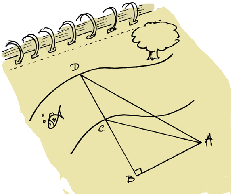
\includegraphics[scale=1]{../medias/1M/trigo/1M-exo-24}
}
\end{minipage}

}
\correction{

}

